\chapter{Tools for DHT and Blockchains}
\section{Cryptographic Tools}
\begin{definition}[Hash Function]
   An hash function converts a binary string of arbitrary length to a binary string of fixed length
\end{definition}

\subsection{Hash functions and collisions}
Non-crypto hash functions have low collision probability, but for an adversary specifically looking to produce one, it may be easy to succeed.\\
For example, the \textit{Cyclic Redundancy Check} (\texttt{CRC}) ---which essentially is the remainder in a long division calculation--- was long mistakenly used where instead crypto integrity was required.
Even if it is unlinkely to generate a collision using random errors, it is reasonably easy for an adversary to find one. 

Note that \ul{collisions \textit{always} exist}, because the codomain is always smaller than the domain of the function.
\note{The \textbf{pigeonhole principle} states that if $n$ pigeons are put into $m$ pigeonholes, with $n > m$, then at least one pigeonhole must contain two or more pigeons.}
The term \textbf{hash security} refers to how hard is to \textit{find} a collision for a given hash function.

\framedt{Birthday Paradox}{
   A hash function $H$ has $n$ possible output bits, so $2^n$ possible output strings.\\
   If $H$ is applied to $k$ inputs, in order to have the probability of a collision greater than $1/2$, $k$ must be greater than $\sqrt{2^n} = 2^{n/2}$.
   This is known as the \textbf{birthday paradox}.
}
\subsection{Cryptographic Hash functions}
{Two main properties must hold for an HF to be cryptographic:\ns
\begin{enumerate}
   \item \textbf{Adversarial collision resistance}
   \item \textbf{One way function}
\end{enumerate}}

{These are formalized as:\ns
\begin{enumerate}
   \item \textit{Pre-image} resistance\\
   $\forall y \in Y. \textit{ hard to find } x \in X\ |\ h(x) = y$
   \note{\textit{``one-way function''}}
   \item \textit{Second pre-image} resistance
   $\textit{given } x \in X, y = h(x). \textit{ hard to find } x' \in X\ |\ h(x') = y$
   \note{Also called \textit{\ul{weak} collision resistance}}  
   \item \textit{Collision} resistance
   $\textit{Hard to find } x_1,x_2 \in X. x_1 \neq x_2 \wedge h(x_1) = h(x_2)$
   \note{Also called \textit{\ul{strong} collision resistance}}
   Given a $m-bit$ hash function, the attacker needs about $2^{m/2}$ brute force computation to find a collision, as stated by the birthday paradox.
\end{enumerate}
}

\subsection{Hiding and Puzzles}
For cryptocurrencies and blockchains also \textbf{hiding} and \textbf{puzzle-friendliness} are required.
\begin{definition}[Hiding]
a hash function $H$ is said to be hiding when a secret value $R$ is chosen from
a probability distribution that has high min-entropy, then, given  $H(R || x)$, it is infeasible to find $x$
\end{definition}
\nl

\framedt{Commit and Reveal} {
   \begin{enumerate}
      \item Alice commits to a value $x$ by sending $H(x)$ to Bob
      \item Alice reveals $x$ to Bob
      \item Bob checks that $H(x)$ matches the commitment
   \end{enumerate}
   Basically the commitment is a \textit{hash} of the value, and the value is revealed after the hash is sent.
   Suppose you have to remotely play Rock-Paper-Scissors: you can both commit to your choice by sending the hash of it, and then reveal them at the same time, resulting in a fair game. 
}

{A hash/search puzzle consists of:\ns
\begin{itemize}
   \item Cryptographic hash function, $H$
   \item Random value, $r$
   \item Target set, $S$
   \item Solution of the puzzle is a value $x$, such that:
   $m = r || x \wedge H(m) \in S$
\end{itemize}}
Bitcoin \textit{Proof of Work} (\textbf{PoW}) is based on a hash/search puzzle.
\begin{definition}[Puzzle friendliness]
   $H$ is said to be puzzle friendly if:
   \begin{itemize}
      \item For every possible n-bit output value $y$, if $r$ is chosen from a distribution with high min entropy, then it is \ul{infeasible to find $x$ such that $H(r || x) = y$ in time significantly less than $2^n$}.
   \end{itemize}
\end{definition}
Puzzle-friendly property implies that
\textit{no} solving strategy to solve a search puzzle is much better than \textit{trying exaustively} all the values $x \in X$.

\subsection{Use cases}
\begin{itemize}
   \item \textbf{Data fingerprinting}\\
   In general $H(x) = H(y) \Rightarrow x = y$, so $H$ allows us to avoid comparing the whole files
   \item \textbf{Message Integrity}\\
   $H(x)$ may be used as a checksum value
   \item \textbf{DHT}s
   \item \textbf{Digital Signature}\\
   Hash functions are widely used for public-key aymmetric algorithms, for ensuring both \textit{confidentaliaty} and message \textit{integrity} (and \textit{authentication}), by appending a \textbf{digest} to the message.
   \note{Recall that without a \textit{digital certificate} proving the identity of the sender, only ``weak authentication'' is provided;
   without one, a third party may impersonate someone else.} 
   The major challenge for digital signatures is to prevent adversaries from learning how to sign messages by analysing the verification-key.
   
\end{itemize}



\section{Data Structures}

\subsection{Bloom Filters}
\textbf{Bloom Filters} answers queries like \textit{``is $k$ an element of $S$''}; they assess the \textit{Set Membership} problem. Bloom filters are fast and lightweight but provide a proabilistic answer
\begin{equation}
   BF(k) = 
   \begin{cases*}
      $0$ & $k \notin S$\\
      $1$ & $k \textit{ \ul{may be} in } S$  
   \end{cases*}   
\end{equation}
Given $n$ elements mapped on $m$ bits through $k$ hash functions, the probability of false positives is
\begin{equation*}
   p' = \left( 1 - \frac{1}{m}\right) ^{kn} \approx e^{-kn/m}
\end{equation*}

A common use of BFs is to perform the \textbf{intersection} between them.
It is possible to compute also the \textbf{union} of two BFs, by computing the Bitwise OR of the two BFs.
\textbf{Delete} operation is not possible, but it is possible to use a \textit{Counting Bloom Filter} to keep track of the number of times an element has been inserted, and increment or decrement the counter accordingly.

Bloom Filters are used by Ethereum, Google, and Bitcoin.

\subsection{Merkle Hash Tree}
\begin{paracol}{2}
   It is a data structure summarizing a big quantity of data, with the goal of verifying the correctness of the content.
   A \textbf{Merkle Hash Tree} consists of a complete binary tree of hashes built starting from an initial set of data:
   \begin{itemize}
      \item $i^{th}$ leaf stores the hash $h_i$ of $f_i$ 
      \item An internal node contains the concatenation of the hashes of the sons of the node
      \item The last hash stored in the root is called \textit{Merkle Root Hash}
   \end{itemize}
   
\switchcolumn

\begin{figure}[htbp]
   \centering
   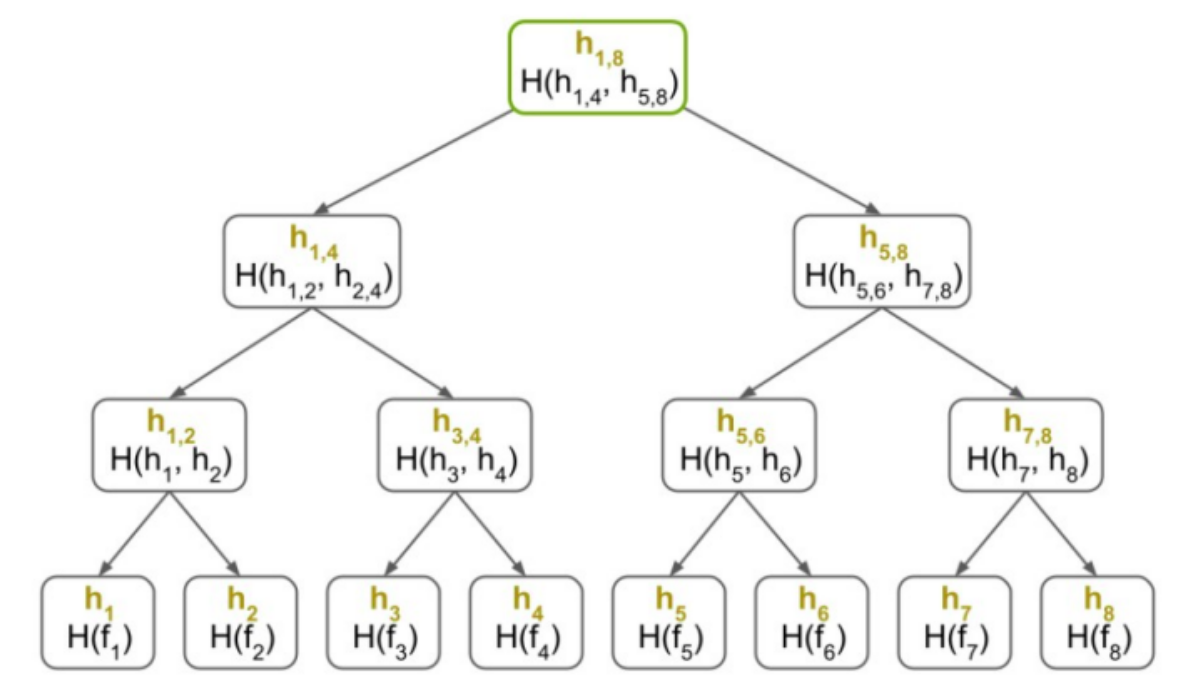
\includegraphics{images/merkle.png}
   \caption{Merkle}
   \label{fig:merkle}
\end{figure}
\end{paracol}

A \ul{collision-resistant hash function \textit{Merkle Hash Tree} (\texttt{MHT}) takes $n$ inputs $(x_1,\dots,x_n)$ and outputs a Merkle root hash $h=MHT(x_1,\dots,x_n)$}. Such function has an important property:
\begin{center}
   Imagine Alice (\textit{verifier}) knows only the Merkle root hash $h$;\\
   Bob (\textit{prover}) can give Alice one of the values $x_i$ and convince Alice that it was the $i^{th}$ input used to compute $h$.
   To convince her, Bob gives Alice an associated Merkle proof without
   showing all the other inputs;
   if a Merkle proof says that $x_i$ was the $i^{th}$ input used to computed $h$, no attacker can come up with another Merkle proof that says a different $x'_i\neq x_i$ was the $i^{th}$ input uses in MHT
\end{center}
\begin{definition}[Merkle Proof Consistency Theorem]
   It is unfeasible to output a Merkle root $h$ and two \textit{inconsistent} proofs $\pi_i$ and
   $\pi'_i$ for two different inputs $x_i$ and $x'_i$ at the $i^{th}$ leaf in the tree of size n
\end{definition}
This can be proved by intuition as follows:
if the proof verification had yielded the same hash but with a different \st{file} leaf
$f'_i\neq f_i$ as the $i^{th}$ input, this would yield a collision in the underlying hash function
$H$ used to build the tree; but such a collision is not possible if $H$ is collision resistant.

The reason to build a Merkle tree is to avoid sending the whole tree to the verifier, but only the path from the leaf to the root, which is logarithmic ($log n$) in the number of leaves.
I case of thousands of leaves, the proof is much shorter than the tree itself.

\subsubsection*{Enlightening Example - Cloud File Integrity}
\begin{figure}[htbp]
   \centering
   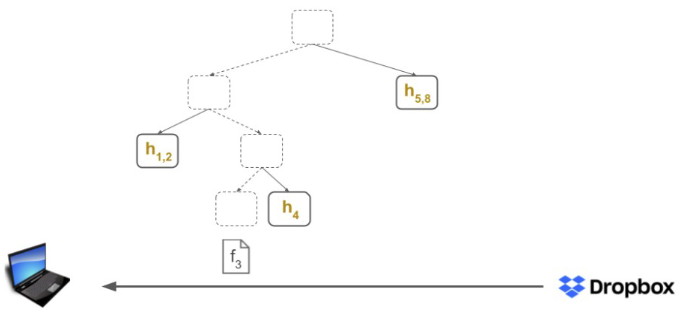
\includegraphics{images/merkle_example.png}
   \caption{Cloud file integrity use case}
   \label{fig:merkle_example}
\end{figure}
Suppose that the user downloads the file f3 ---which was earlier on stored on the user's PC--- and wants to check that Dropbox hasn't tampered/corrupted it.
The user must keep only the \textbf{hash root} of the file they had uploaded on Dropbox, not the whole Merkle Tree.\\
Dropbox can provide ---along with the file--- a portion of the original Merkle Tree (the \textit{Merkle Proof} or \textit{Membership proof}), only the nodes needed for the user to compute the Merkle proof, i.e. computing the sequence of hashes ``filling the blanks'' up to the root and check that the resulting root matches the one stored on the user's PC.
\note{I think that the Dropbox cannot fake a Merkle tree by choosing fake $h_4,h_{1,2}, h_{5,8}$ such that the root is the one expected by the user, due to the \textit{collision resistant} property of $H$}

\section{Tries and Patricia Tries}
\begin{paracol}{2}
   \colfill
   \labelitemize{\textbf{\textit{Trie}}}{
      \begin{itemize}
      \item The root node stores nothing.
      \item Edges are labeled with letters and a path from the root to the node
      represents a string.
      \item The nodes come with an indicator, which indicates whether that node
      represents the end of a string.
      \end{itemize}
   }
   
   This is very space consuming since every node stores a label. 
   The trie may be compressed by storing only the first different prefixes\footnotemark[1]  in the nodes, resulting in an equivalent \textbf{Patricia Trie}, shown in the second figure.
   \colfill
   \switchcolumn
   
   \begin{figure}[htbp]
      \centering
      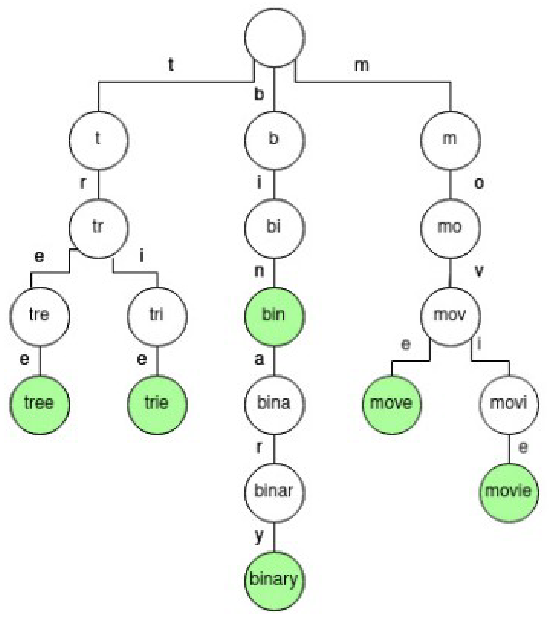
\includegraphics[width=0.60\columnwidth]{images/trie.png}\\
      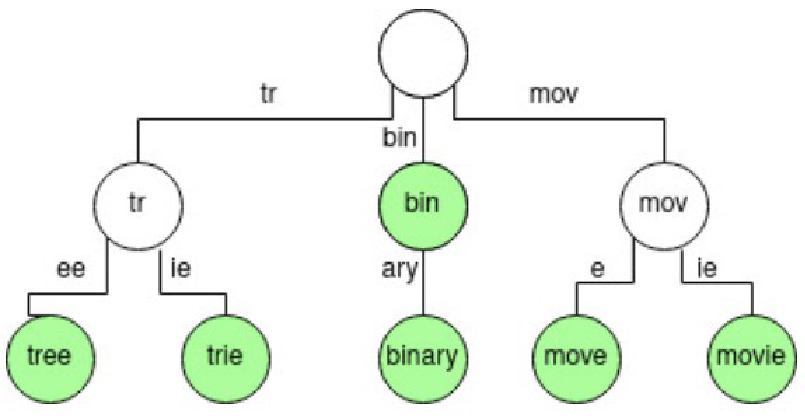
\includegraphics{images/patriciatrie2.png}
      \caption{Trie and corresponding Patricia Trie}
      \label{fig:trie}
   \end{figure}
\end{paracol}

\subsection{Patricia Merkle Trie}

\begin{figure}[htbp]
   \centering
   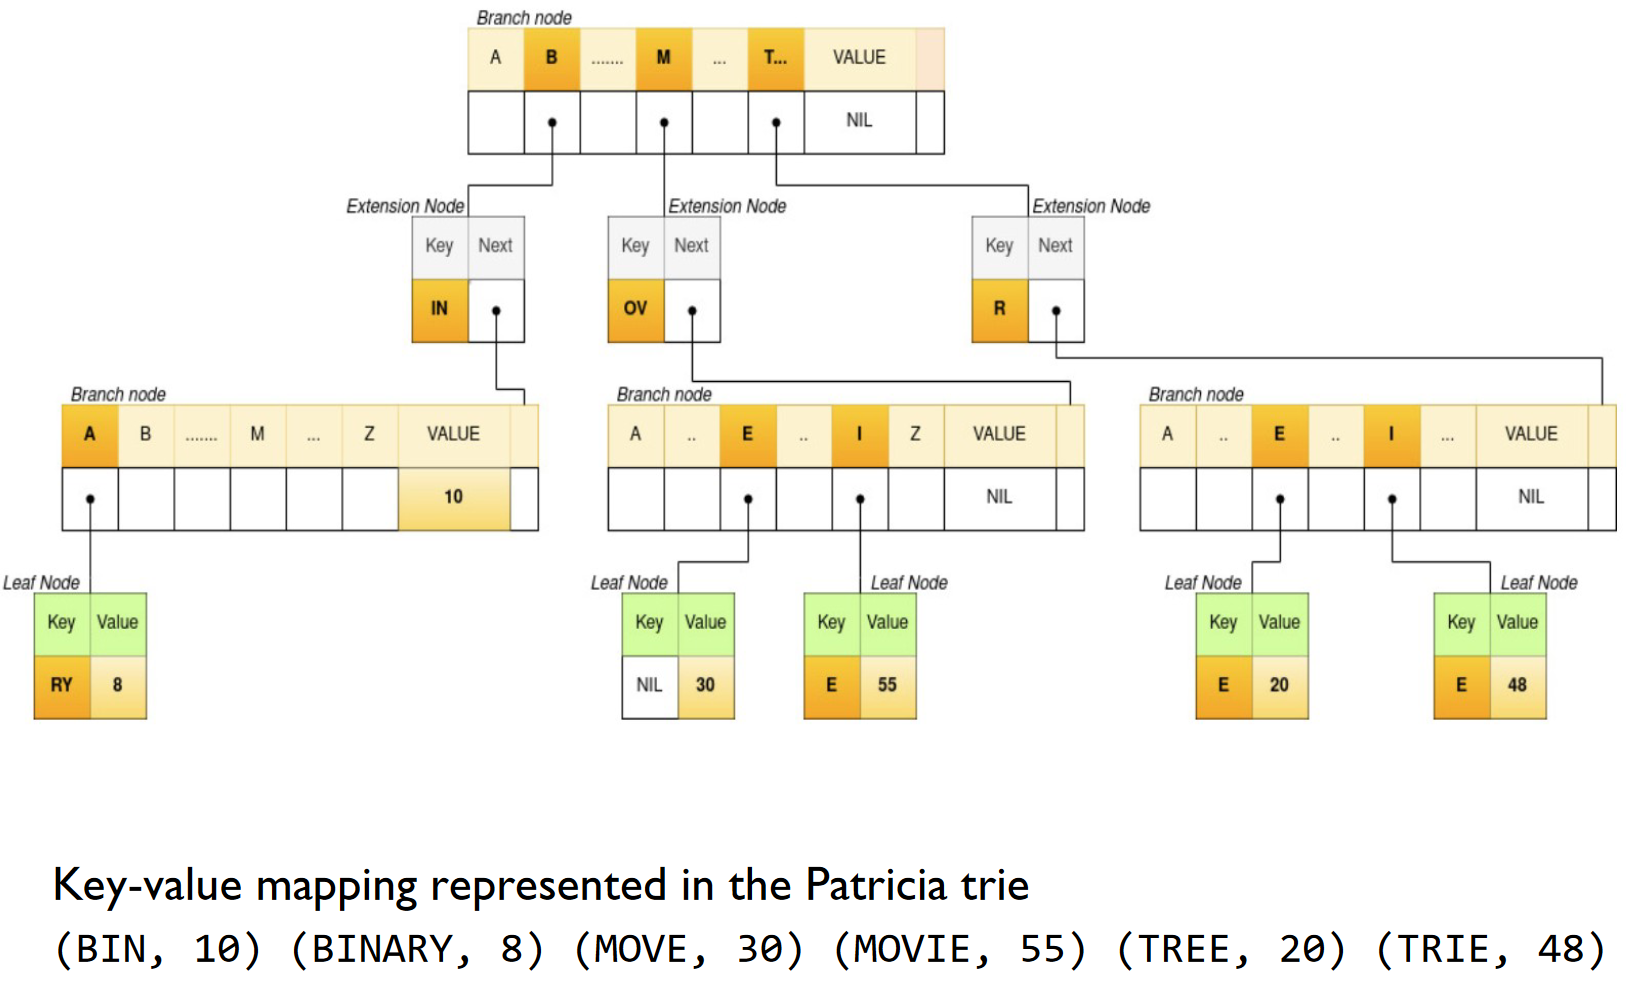
\includegraphics{images/patriciaMerkle.png}
   \caption{Patricia Merkle \textit{key-value} Trie}
   \label{fig:patriciaMerkle}
\end{figure}
A \textbf{Patricia Merkle Trie} is a combination of a Merkle Tree and a Patricia Trie, introduced by Ethereum.
{Nodes may be of three types:\ns
\begin{enumerate}
   \item \textit{Branch} Node - multiple children, and may store a \textbf{value} referred to the key which points to such Branch Node (if it is indeed a key and not a prefix)
   \item \textit{Extension} Node - single child, and stores the \textbf{prefix} of the key
   \item \textit{Leaf} Node - stores the final bits of the \textbf{key} and the \textbf{value}
\end{enumerate}
}

A trie can be used to store a set of key-value pairs, where the key is a string and the value is either a pointer to another child (or node), or the value itself, in case of a leaf node.

{In Ethereum the Patricia Merkle Trie is used to store the state of the blockchain, where the \ul{key} is the address of \ns
\begin{enumerate}
   \item an \textit{account} and the \ul{value} is the account \textit{balance}.
   \item a \textit{transaction} and the \ul{value} is the \textit{transferred amount}.
\end{enumerate}}

{Since the nodes of such tree are multi-element, and hash functions are instead applied to strings, some sort of \textbf{serialization} is applied: \ns
\begin{itemize}
   \item \texttt{HP} - \texttt{Hex Prefix Encoding} for the keys
   \item \texttt{RLP} - \texttt{Recursive Length Prefix Encoding} for the values (which may be \textit{structured data})
\end{itemize}}

\footnotetext[1]{Actually also only the first different character should be ok, if I recall corecctly from Algorithm Engineering course}